\documentclass[border=10pt]{standalone}
\usepackage{tikz}\usepackage{amsmath}\usetikzlibrary{arrows.meta,patterns}
\begin{document}
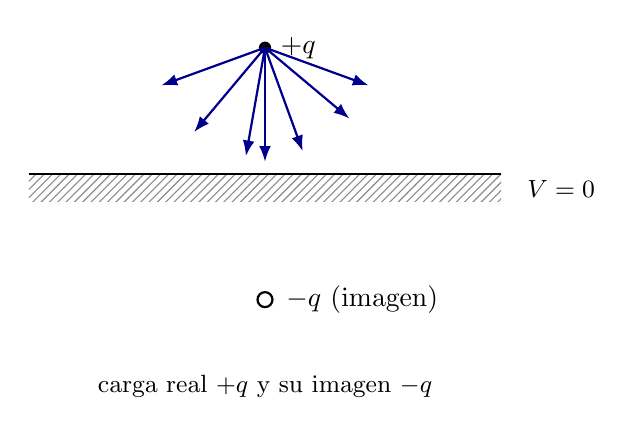
\begin{tikzpicture}[line width=0.8pt,>={Latex[length=2mm]}]
  \fill[pattern=north east lines,pattern color=black!45] (-3,-0.35) rectangle (3,0);
  \draw[thick] (-3,0)--(3,0);
  \node at (3.2,-0.2)[right]{\small $V=0$};
  \fill (0,1.6) circle(2.2pt) node[right=2pt]{$+q$};
  \draw[fill=white] (0,-1.6) circle(2.7pt);
  \node at (0,-1.6)[right=4pt]{$-q$ (imagen)};
  \foreach \a in {200,230,260,290,320,340}
     \draw[->,blue!55!black] (0,1.6)--+(\a:1.4);
  \draw[->,blue!55!black] (0,1.6)--(0,0.15);
  \node at (0,-2.7){\small carga real $+q$ y su imagen $-q$};
\end{tikzpicture}
\end{document}
